% SPDX-License-Identifier: Apache-2.0
\section{Optionale Erwerbs- und Zeitplanung: Reihenfolge und Budget}
\label{sec:levels}
Dieser Abschnitt beantwortet zwei Planungsfragen: Lassen sich die Ziele
eines Plans in der vorgesehenen zeitlichen Reihenfolge überhaupt erwerben,
und reicht die verfügbare Zeit dafür? Beide Prüfungen rechnen mit einem
Plan, nicht mit dem Lernzustand einer Person.

\begin{principle}{Status: zusätzliches Planungsprofil}
Lerneinheiten tragen den fachlichen Zusammenhang und ihren rekursiven
Abschluss. Ein optionaler Zeitplan ordnet deren Erwerbsziele auf
Planungsstufen, etwa Schuljahre oder Semester, und prüft verfügbare Zeit.
Diese Zuordnung ist keine Definition der Lerneinheiten. Sie verändert weder
Grundgraphgültigkeit noch gespeicherte Mastery und führt keine technischen
Einheitssperren ein. Ein produktiver neuer Budgetvalidator wird nicht behauptet.
\end{principle}

Eine fachliche Einheit kann in verschiedenen Bildungsgängen zu anderen
Zeiten erworben werden. Eine Planungsstufe bezeichnet hier nur einen
geplanten Zeitraum, bildhaft eine Bauetappe: Kompetenzen bleiben die
Bauteile, und ihre fachlichen Voraussetzungen bleiben erhalten. Es folgt
daraus keine Pflicht, erst alle Fächer eines Kalenderjahres abzuschließen,
bevor irgendein späteres Ziel zugänglich wird.

\subsection{Plan, Eintrittsbasis und eindeutiger Ersterwerb}
Für einen aufgelösten Plan $\pi$ seien
\begin{align}
 T_\pi&\subseteq A &&\text{geplante Erwerbsziele},\\
 B_\pi&\subseteq A\setminus T_\pi &&\text{ausdrücklich angenommene Eintrittsbasis},\\
 n_\pi&\in\N_{>0},\qquad
 \ell_\pi:T_\pi\to\{1,\ldots,n_\pi\} &&\text{Planungsstufe}.
\end{align}
Der Plan nennt also, was erworben werden soll ($T_\pi$), was beim Eintritt
als vorhanden angenommen wird ($B_\pi$) und in welcher der $n_\pi$
Planungsstufen jedes Ziel erstmals erworben wird ($\ell_\pi$).
Die Planungsstufen und ihre Präfixe sind
\[
 S_i=\{g\in T_\pi\mid\ell_\pi(g)=i\},\quad
 S_{<i}=\bigcup_{j<i}S_j,\quad S_{\leq i}=\bigcup_{j\leq i}S_j.
\]
Diese zeitliche Zuordnung (Abbildung~\ref{fig:levels}) referenziert die
fachliche Ersterwerbszuordnung der Lerneinheiten, ersetzt sie aber nicht. Jedes Ziel wird im Plan
einer ersten Planungsstufe zugeordnet. Ein anderer
Bildungsgang darf es anders platzieren. Spätere Wiederholung, Vertiefung oder
Anwendung sind zusätzliche Aktivitäten, keine neue Zielidentität.
$B_\pi$ ist eine Planungsannahme; sie schreibt keine Lernergebnisse.
Persönliche Lücken in dieser Basis brauchen eine eigene Diagnose und
zusätzliche Lernzeit.

\begin{figure}[htbp]\centering
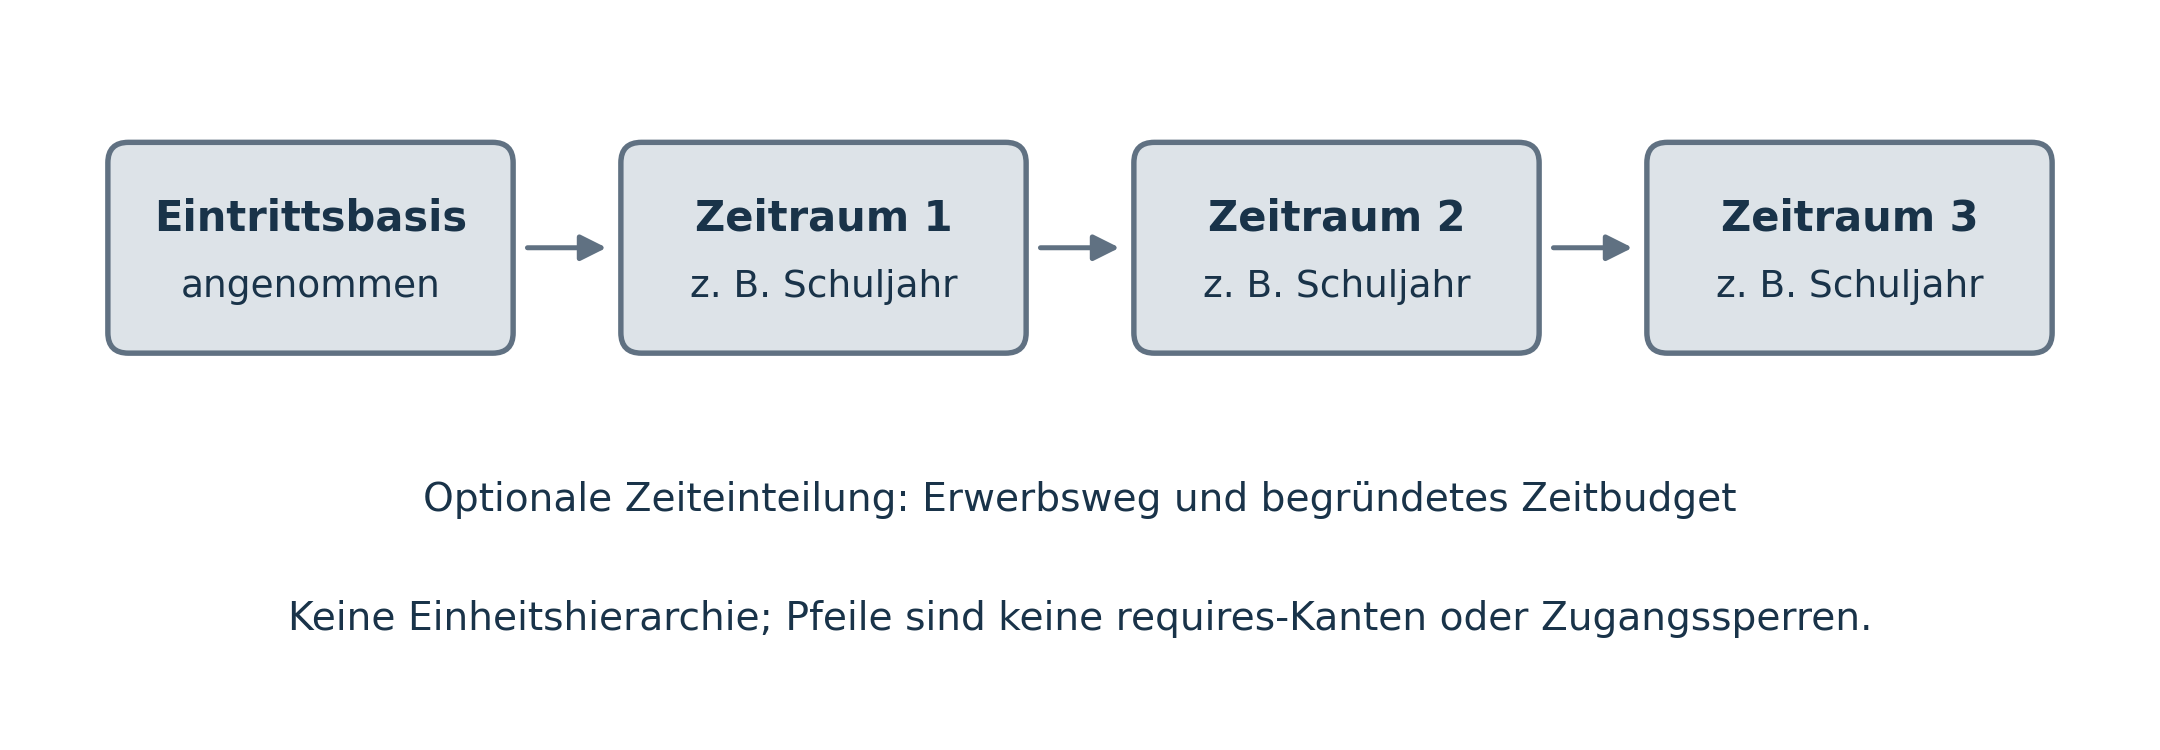
\includegraphics[width=.85\linewidth]{assets/graph-definition/12-calendar-planning.png}
\caption[Optionale kalenderbezogene Planungsstufen]{Die zeitliche
Reihenfolge ist keine rekursive Einheitshierarchie. Pfeile sind keine
\code{requires}-Kanten und führen keine Zugangssperren ein.}
\label{fig:levels}\end{figure}

\subsection{Strukturelle Machbarkeit durch einen Abschlusszeugen}
\label{sec:witness}
Die angenommene Eintrittsbasis setzt eine Planungsgrenze: Ihre frühere
Erwerbsgeschichte wird nicht rekonstruiert. Nur für den hypothetischen
Planungstest sei deshalb
\[
 \Rat^{\pi}=\{(a,b)\in\Rat\mid a\notin B_\pi\}.
\]
$\Frontier_\pi$ ist die Frontier aus \eqref{eq:frontier} mit dieser
Relation und ihrer vollständigen transitiven Hülle. Alle Ziele und früheren
Planungsstufen behalten ihre transitiven Anforderungen; nur an deklarierten
Eintrittskompetenzen endet die Planungsrekonstruktion. Diese Ausnahme
erlaubt keinen Stopp an Mastery-Zwischenzielen im wirklichen Lernzustand.

Ein \emph{Abschlusszeuge} einer Planungsstufe ist eine Reihenfolge ihrer
Ziele, in der jedes Ziel verfügbar ist, sobald es an der Reihe ist.
Eine Planungsstufe $S_i$ mit $s_i$ Zielen ist strukturell machbar, wenn
sich ihre Ziele als $a_1,\ldots,a_{s_i}$ aufzählen lassen, sodass
\begin{equation}
 a_j\in\Frontier_\pi\!\left(B_\pi\cup S_{<i}\cup
                         \{a_1,\ldots,a_{j-1}\}\right)
 \qquad(1\leq j\leq s_i).
 \label{eq:level-witness}
\end{equation}
Setzt etwa $g$ das Ziel $p$ voraus, liegen beide in derselben
Planungsstufe und sind ihre übrigen Voraussetzungen schon erfüllt, dann ist
die Reihenfolge $p,g$ ein Abschlusszeuge, die Reihenfolge $g,p$ nicht.
Hier gilt der globale Prüfbereich. Vererbte, clusterbezogene und nach
Referenzauflösung fachübergreifende Anforderungen bleiben erhalten.
Ein Normalmodusfilter würde relevante Anforderungen ausblenden können.
Der hypothetische Abschlusszeuge verwendet keine direkten Prüfungssprünge
und nimmt keine implizite Anerkennung vorweg.

Zur Diagnose dienen die benötigten Atome, also der atomare Bedarf aus
\eqref{eq:demand} bezüglich der Planrelation:
\begin{equation}
 \ReqAtoms_\pi(g)=\{b\in A\mid(g,b)\in(\Rat^{\pi})^+\}.
 \label{eq:reqatoms}
\end{equation}
Aus einem Abschlusszeugen folgt notwendig
\begin{equation}
 \forall g\in T_\pi:\quad
 \ReqAtoms_\pi(g)\subseteq B_\pi\cup S_{\leq\ell_\pi(g)}.
 \label{eq:level-closure}
\end{equation}
Jedes benötigte Atom liegt also in der Eintrittsbasis oder wird spätestens
in derselben Planungsstufe erworben. Eine benötigte Kompetenz außerhalb
$B_\pi\cup T_\pi$ ist ungeplant;
ein benötigtes Ziel mit höherer Planungsstufe ist ein Reihenfolgefehler.
Voraussetzungen innerhalb derselben Planungsstufe sind erlaubt. Die
Grundgraphgültigkeit einschließlich atomar expandierter Zyklen muss vor
dieser Mengenprüfung bereits festgestellt sein. Der explizite Zeuge
verbindet die Zuordnung mit einem tatsächlich möglichen Erwerbsweg.

Ein endlicher Prüfalgorithmus startet für jede Planungsstufe mit dem
hypothetischen Stand $W^{(0)}=B_\pi\cup S_{<i}$ und wiederholt
\begin{equation}
 W^{(r+1)}=W^{(r)}\cup\bigl(S_i\cap\Frontier_\pi(W^{(r)})\bigr).
\end{equation}
Er ist erfolgreich genau dann, wenn sein Fixpunkt ganz $S_i$ enthält.
Die Verfügbarkeit eines noch offenen Ziels kann durch zusätzliche
Erfüllungen nicht verschlechtert werden. Deshalb kann jede gleichzeitig
hinzugefügte Menge auch nacheinander erworben werden. Ein vorhandener
Abschlusszeuge kann umgekehrt nicht vorzeitig an diesem Verfahren scheitern.
Das Verfahren ist ein \emph{hypothetischer} Lerndurchlauf; es ändert keine
persönlichen Daten. Im rein atomaren DAG liefert eine voraussetzungsgetreue
topologische Ordnung den bekannten Spezialfall.

\subsection{Aufwand, Reserve und Budget}
Strukturelle Machbarkeit beweist noch nicht, dass ein Schuljahr zeitlich
ausreicht. Jede Zeitbehauptung nennt Referenzlernende, Eintrittsbedingungen,
Ziel- und Wahlauswahl, Kalender, Schätzmethode und Unsicherheit.
Diese deklarierten Schätzannahmen des Plans $\pi$ fassen wir als
$\Theta_\pi$ zusammen. Für eine tatsächliche Aktivität $h$ bezeichnet
$\widehat t_h(\Theta_\pi)\geq0$ ihre unter diesen Annahmen geschätzte Dauer.
Alle Größen müssen in derselben kalibrierten Zeiteinheit vorliegen:
\begin{equation}
 \Work_\pi(i;\Theta_\pi)+\Reserve_\pi(i)\leq \Budget_\pi(i),
 \qquad i=1,\ldots,n_\pi.
 \label{eq:budget}
\end{equation}
Dabei sind $\Work\geq0$, $\Reserve\geq0$ und $\Budget>0$.
Reserve ist geschützt und wird nicht gleichzeitig als verplanbare Zeit
ausgegeben. Ein Nullpuffer ist möglich, aber offenzulegen. Bereits im
Arbeitsaufwand enthaltene Prüfungsvorbereitung oder Wiederholung darf nicht
ein zweites Mal als Reservebedarf gezählt werden.

Ein erklärtes Aktivitätenmodell kann
$\Work_\pi(i;\Theta_\pi)=\sum_{h\in\mathcal H_i}\widehat t_h(\Theta_\pi)$
verwenden. $\mathcal H_i$ enthält jeden tatsächlichen Aufwand genau einmal:
Ersterwerb, gezielte Übung, Abruf, Prüfung und weitere geplante Arbeit.
Dasselbe kanonische Atom wird nicht in Mathematik und Physik zweimal als
Ersterwerb gezählt; eine zusätzliche Anwendung in Physik kann dennoch
eigenständige Zeit kosten. Unkalibrierte \glqq Zielpunkte\grqq{} oder
\code{weight}-Werte sind keine Minutenschätzung.
Tabelle~\ref{tab:workload} veranschaulicht die getrennte Verbuchung von
Arbeit und Reserve.

\begin{table}[htbp]
\centering
\begin{tabular}{@{}lrr@{}}
\toprule
Illustrative Planung & Stunden & Bedeutung\\
\midrule
Ersterwerb & 42 & Bereits um gemeinsame Ziele bereinigt\\
Übung und Anwendung & 12 & Zusätzliche Tätigkeiten\\
Prüfung und Wiederholung & 6 & Im Arbeitsaufwand enthalten\\
Geschützte Reserve & 10 & Nicht für obige Arbeit verplant\\
Verfügbare Zeit & 75 & Nach Kalenderausschlüssen\\
\bottomrule
\end{tabular}
\caption{Rechenbeispiel: $\Work=60$ und $\Reserve=10$ passen in
$\Budget=75$. Die erfundenen Zahlen demonstrieren nur die Rechnung,
keine empirisch abgesicherte Dauer eines SkillPilot-Curriculums.}
\label{tab:workload}
\end{table}

Ein Gesamtbudget genügt nicht, wenn Fächer, Räume oder Termine eigene
bindende Grenzen haben. Für eine zusätzlich deklarierte Fächerzuordnung
müssen auch die jeweiligen $\Work_{i,s}+\Reserve_{i,s}\leq \Budget_{i,s}$
gelten, ohne Doppelzählung gemeinsam zugeordneter Zeit. Ein Kalenderplan
muss außerdem Voraussetzungen vor der konkreten Anwendung bereitstellen.

\subsection{Gültigkeitsanspruch und Abschlussgrenzen}
Ein Zeit- und Erwerbsplan ist unter diesem optionalen Profil gültig, wenn
er sowohl strukturell als auch unter seinen erklärten Annahmen zeitlich
machbar ist.
Ohne belastbare Aufwandsschätzung ist allein die strukturelle Aussage
zulässig. Der Anspruch bindet Plan, Curriculumfassung, aufgelösten Umfang
und Schätzannahmen. Er garantiert keine identische Lerngeschwindigkeit
für jede Person.

Der Abschluss der fachlichen Lerneinheit folgt den rekursiven Zieltyp- und
Kinderpflichten aus Abschnitt~\ref{sec:learning-units}. Ein Kalenderabschnitt
kann mehrere Einheiten enthalten; eine Einheit kann sich über mehrere
Kalenderabschnitte erstrecken. Aus diesem Zeitprofil folgt keine pauschale
Voraussetzung des gesamten vorigen Jahres für jedes spätere Lernziel.

\sources{%
\srcref{docs/concept/skill-graph/learning-units.md}{Lerneinheiten};
\srcref{docs/concept/skill-graph/graph-definition.md}{Graph Definition, Abschnitt 12};
\srcref{docs/concept/didactic/curriculum-time-axis-and-pacing.md}{Zeitachse und Kapazität}.}
